\documentclass[11pt,a4paper]{article}
% \documentclass[a4paper]{article}
% \usepackage[brazil]{babel} % carrega portugues brasileiro
\usepackage[utf8]{inputenc}
\usepackage[T1]{fontenc}
\usepackage[top=2cm, bottom=2cm, left=2cm, right=2cm]{geometry} %margens menores!
\usepackage{graphicx} % incluir figuras .eps
\usepackage{tabularx}
\usepackage{color} % colorir texto
\usepackage{indentfirst}
\usepackage{textcomp}
\usepackage[colorlinks=true]{hyperref}
\usepackage{amssymb,amsmath}
\usepackage{float}
\usepackage{wrapfig}
% \usepackage{siunitx}
% \usepackage[ampersand]{easylist}

\title{User Manual}


\author{
       \large
       \mbox{Rhizomatica} \\
       \mbox{}\\ 
       \textsc{Rafael Diniz}
        rafael@rhizomatica.org\\
%        \normalsize
%        we want the airwaves
%        \texttt{Brasília - Brasil}\\
}
\date{\today}

\begin{document}

\maketitle

\begin{figure*}[!ht]

\includegraphics[width=1\textwidth]{pictures/logoh.png}
\end{figure*}

\begin{abstract}

  High-Frequency Emergency and Rural Multimedia Exchange System (HERMES) testing procedure for the sBitx v2 radio.

\end{abstract}

\newpage

\tableofcontents

\setlength{\parindent}{0em}
\setlength{\parskip}{1em}

\section{Introduction}

Steps for testing:

\begin{itemize}
\item Connecting RF (Radio Frequency) test equipment
\item Connecting to power supply
\item Initial setup for boot over USB
\item HERMES installer setup
\item Installation procedure
\end{itemize}

%\begin{figure*}[!ht]
%
\includegraphics[width=1\textwidth]{pictures/hermes.png}
%\end{figure*}

\section{Connecting RF test equipment}

For proper testing, the radio needs to be connected, ideally, to a power meter (also called wattmeter), which should be connected to a dummy load, as shown in Figures \ref{fig:backview1}, \ref{fig:backview3}
and \ref{fig:backview2}.

\begin{figure}[!ht]
  \centering
  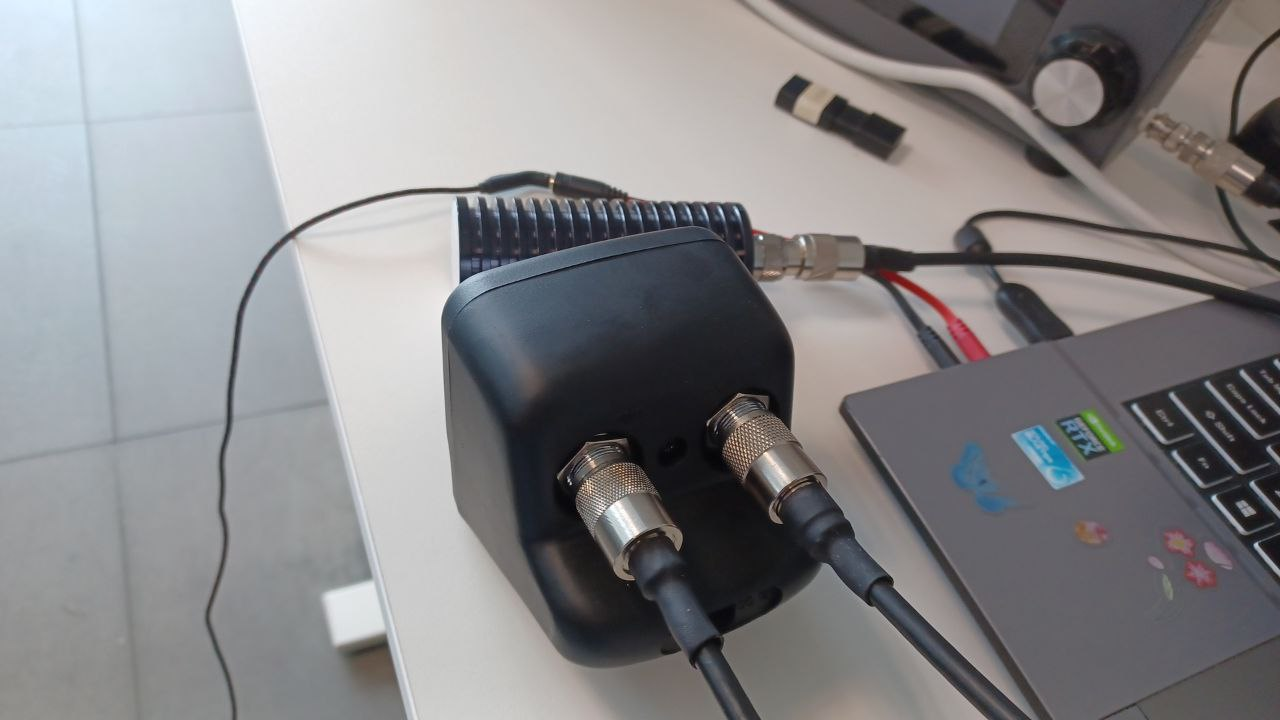
\includegraphics[width=0.5\textwidth]{pictures/wattmeter_1.jpeg}
  \caption{Back of the power meter with the cables attached}
  \label{fig:backview1}
\end{figure}

\begin{figure}[!ht]
  \centering
  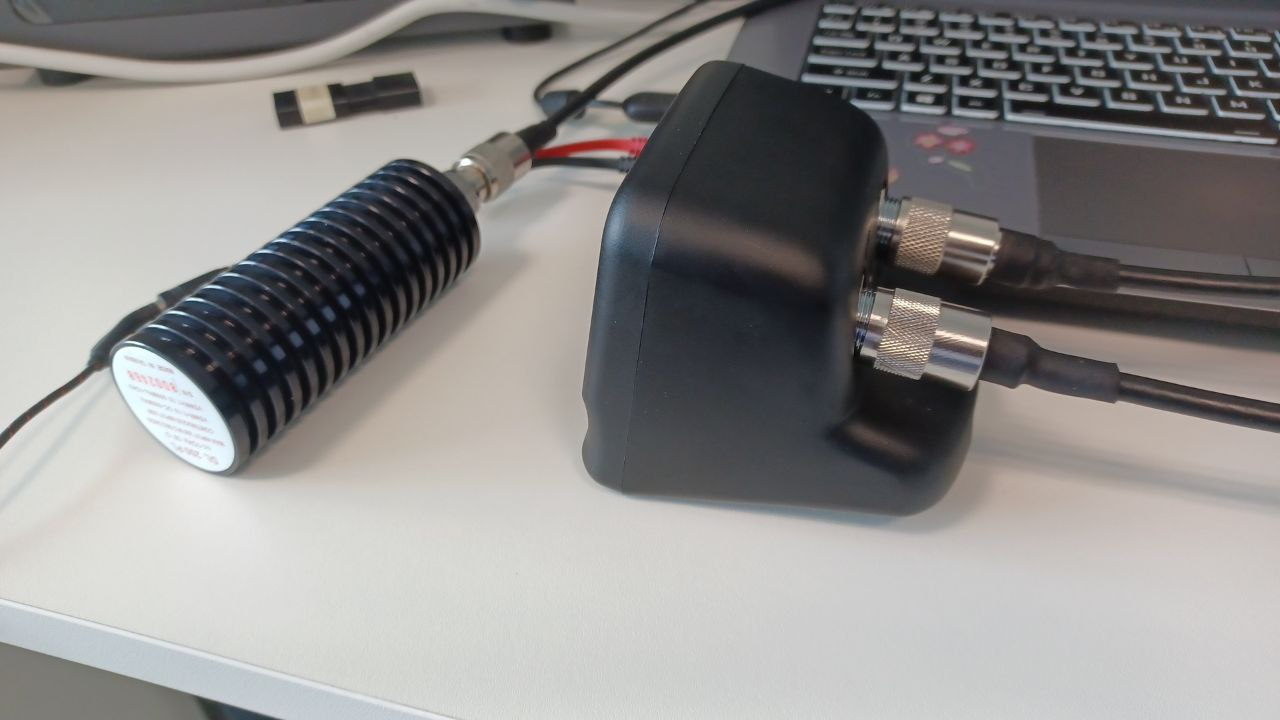
\includegraphics[width=0.5\textwidth]{pictures/wattmeter_3.jpeg}
  \caption{Both the dummy load (left) and the power meter (right)}
  \label{fig:backview3}
\end{figure}


The radio (sBitx v2) has a BNC female connector, and need the appropriate cables and adapters to
be connected to the Wattmeter and dummy load. The wattmeter measures the forward and reflected power of the radio,
and the dummy load simulates an antenna without radiating the signal.

The radio needs to be connected (see Figure \ref{fig:backview4}) to the ``TX'' or ``Transmitter'' (see Figure \ref{fig:backview2}) port of the power meter, while the dummy load
should be connected to the ``ANT'' or ``Antenna'' port.

\begin{figure}[!ht]
  \centering
  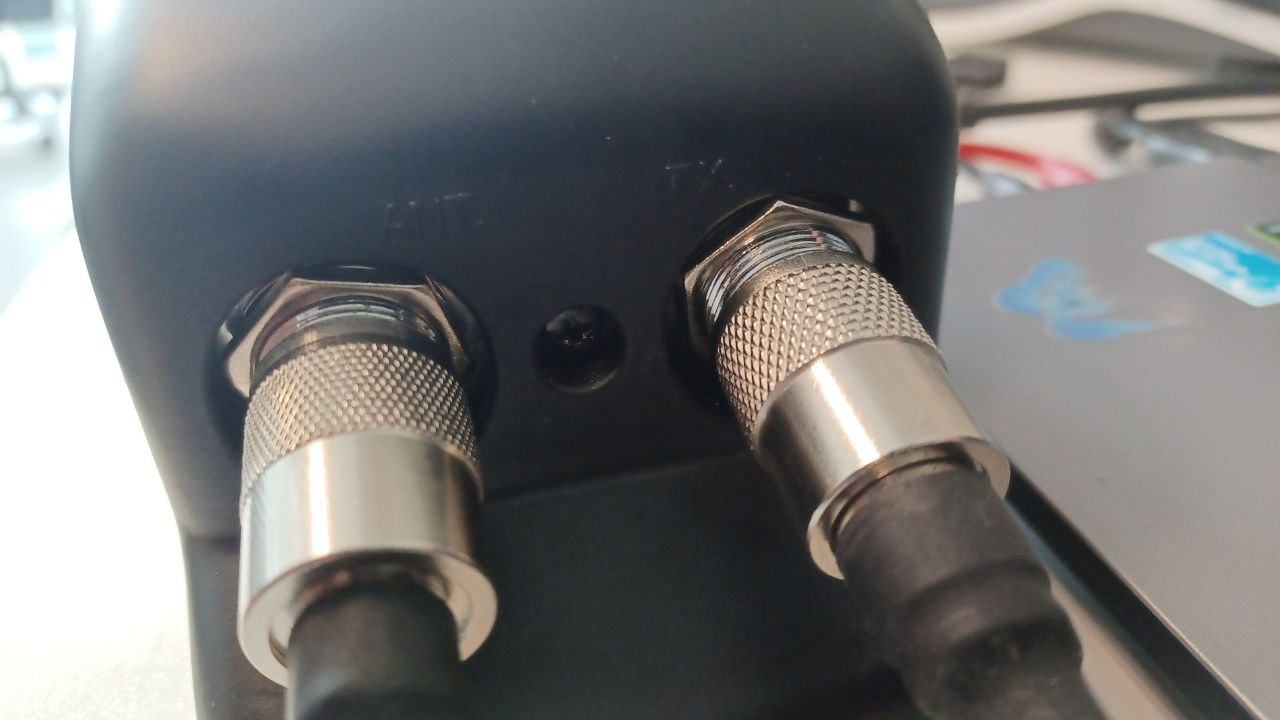
\includegraphics[width=0.5\textwidth]{pictures/wattmeter_2.jpeg}
  \caption{Back of the power meter in which the ANT and TX writings can be seen}
  \label{fig:backview2}
\end{figure}

\begin{figure}[!ht]
  \centering
  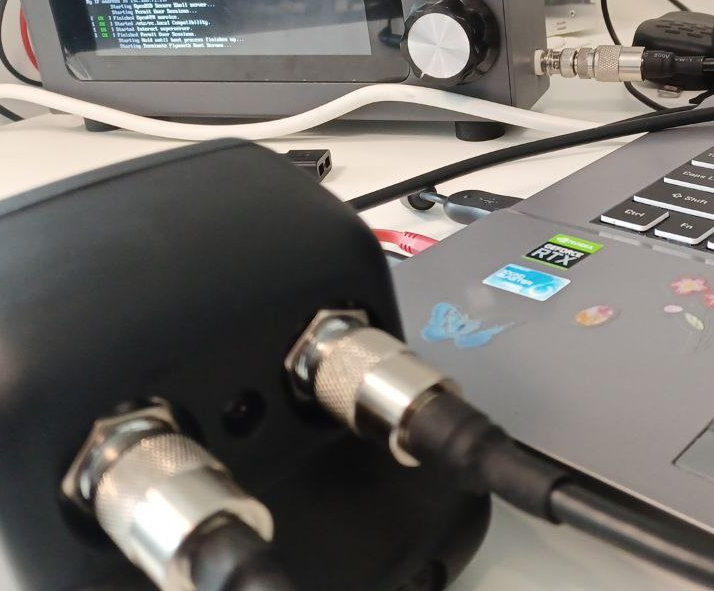
\includegraphics[width=0.5\textwidth]{pictures/wattmeter_4-edited.jpeg}
  \caption{The power meter (left) and radio with the connected cable (top right)}
  \label{fig:backview4}
\end{figure}

Make sure the cables are properly connected and the front of the power meter (Figure \ref{fig:frontview1})
is in a visible position.

\begin{figure}[!ht]
  \centering
  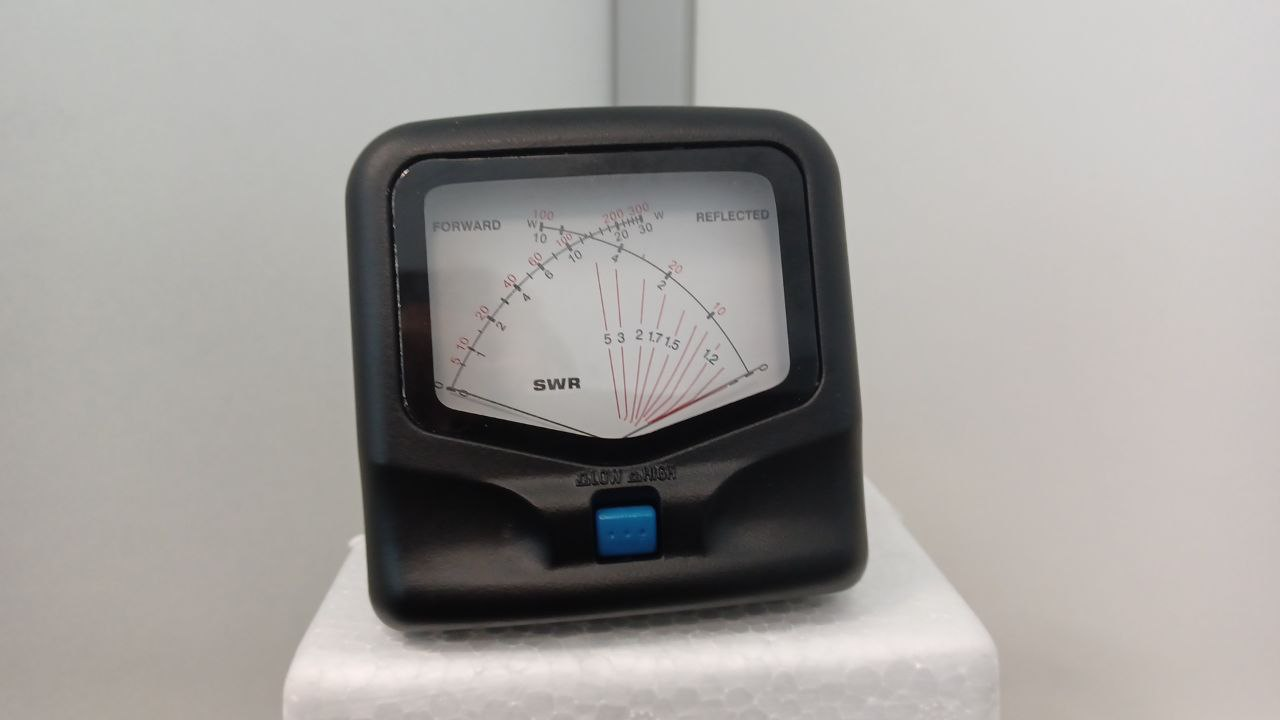
\includegraphics[width=0.5\textwidth]{pictures/wattmeter_5.jpeg}
  \caption{Front view of a power meter}
  \label{fig:frontview1}
\end{figure}

\section{Connecting to power supply}

In order to connect the radio to the power source, a power cable is provided. One side of the
cable comes with a XT60 connector and connects to the radio, and the other end is bare ended,
and should be connected to the positive (Red) and negative (Black) of a 12V battery system, or power
supply.

% put pics...

\section{Initial setup for boot over USB}

First connect a USB keyboard to the radio. and the network (RJ45) cable with appropriate Internet connexion.
Then click in the Terminal icon shown in Figure~\ref{fig:terminal}.

\begin{figure}[!ht]
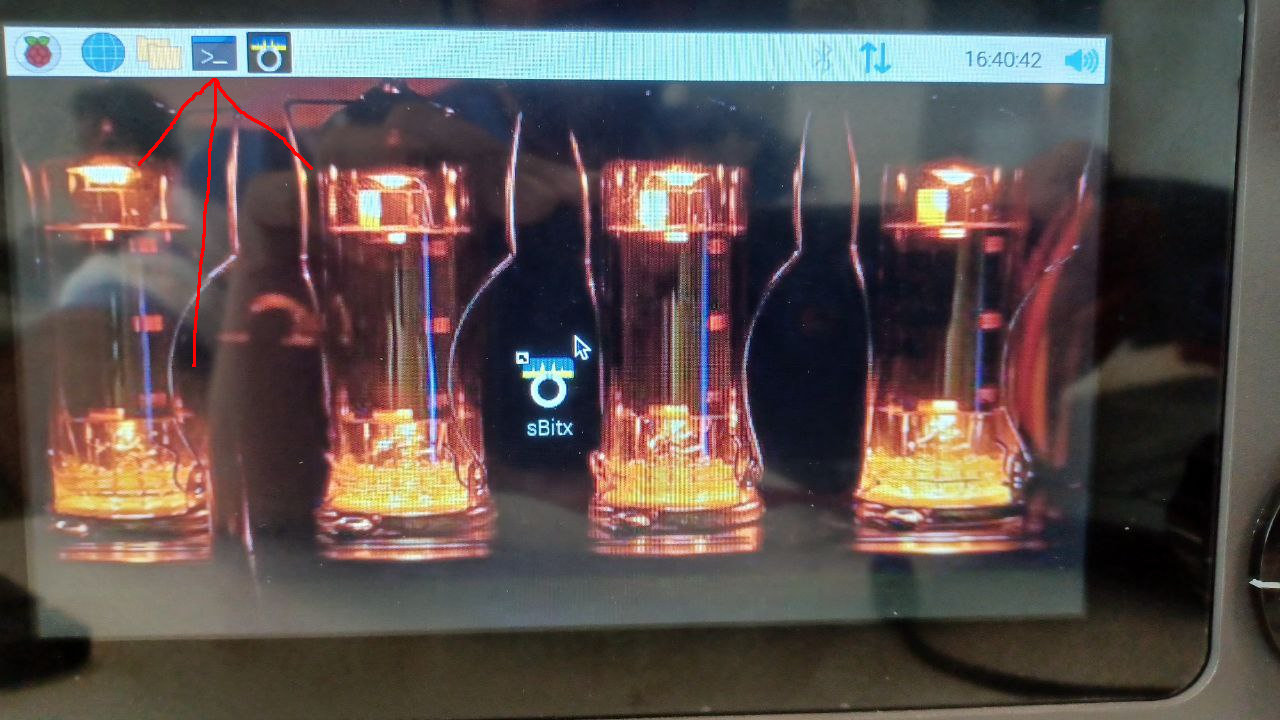
\includegraphics[width=1\textwidth]{pictures/screen1-edited.jpeg}
\caption{Screen of the radio and the ``Terminal'' icon pointed by an arrow}
\label{fig:terminal}
\end{figure}

After opening the terminal window, type:

\begin{itemize}
\item sudo su
\item apt-get update
\item apt-get install rpi-eeprom
\item raspi-config
\end{itemize}

At this point the screen shown in Figure~\ref{} should appear.

Choose the following path in the menu (navigation using arrow and Tab keys):
\begin{itemize}
\item Option 6 (Advanced Options)
\item . Option A6 (Boot Order)
\item . Option B2 (USB Boot)
\item . Finish
\end{itemize}




% default password... root /

\end{document}
